\chapter{Using Mesquite in Parallel}
\label{sec:parallel}

\section{Introduction}

Large meshes are often partitioned across many parallel processors either because they are too large to fit into the memory of a single machine or in order to speed up the computation. Even if it would be possible to assemble all partitions on a single processor, smooth the mesh, and repartition the result, such an approach would be very I/O inefficient. Moreover, for larger meshes such an approach would quickly run out of memory and fail. Therefore Mesquite supports smoothing meshes in parallel.

Mesquite currently does only synchronous Nash-game or local optimizations in parallel \cite{Fr95}.  It does not yet provide parallel solvers and therefore cannot do either block coordinate descent or truly global optimizations in parallel (minimization of an explicit, global objective function.)

For algorithms such as Laplacian smoothing that are local optimizations, optimization in parallel is essentially the same as in serial.  For other optimizations that do a global minimization of an explicitly defined objective function in serial (for example \texttt{ShapeImprover}), the parallel optimization will be a Nash-game type optimization where the interior vertices (those not on the partition boundaries) will be optimized as a group.  Each vertex on the partition boundary will then be optimized individually.  While a global optimization in serial will typically have only one outer iteration, it is generally desirable to do multiple outer iterations in parallel so the Nash-game type optimization can reach convergence.  Mesquite wrappers (see Chapter \ref{sec:wrappers}) that implement global optimizations in serial default to 10 outer iterations in parallel.


\section{Distributed Mesh}

The input mesh for use in parallel quality improvement must be partitioned based on vertices.  That is, each vertex in the mesh must be assigned a single processor as its owner.  For optimal performance, vertices should be evenly distributed amongst available processors and the vertices assigned to the same processor should compose a contiguously connected patch of mesh.

Each processor must also have access to all elements for which the position of its vertices influence the quality.  For almost all algorithms in Mesquite, this is the set of all elements that contain one of the vertices.  Further, each processor must also be able to access any additional vertices owned by other processors that are necessary to define those elements.  The instances of such vertices on processors that do not own them are typically referred to as ``ghosted'' vertices.  Elements for which copies exist on multiple processors may sometimes also be referred to as ``ghosted'' or ``ghost'' elements.

\begin{figure*}[htbp]
\begin{center}
    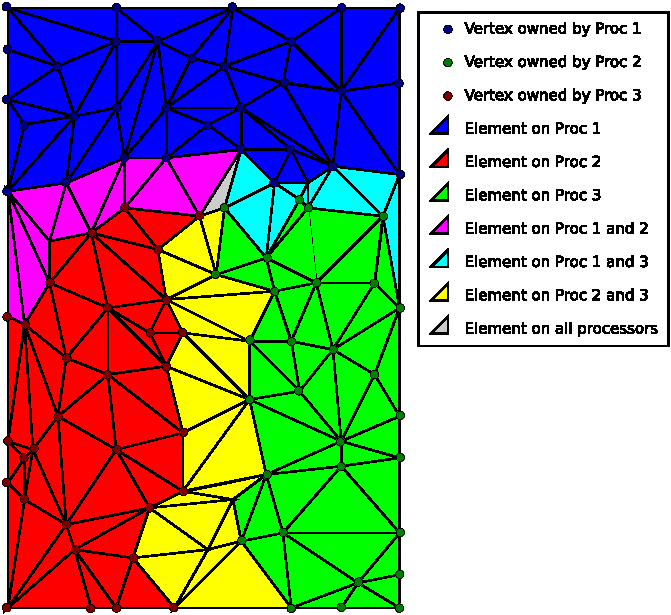
\includegraphics{figures/parallel_mesh}
    \caption{Sharing or ghosting of elements and vertices in a partitioned mesh.}
    \label{fig:parallel_mesh}
\end{center}
\end{figure*}

Figure \ref{fig:parallel_mesh} shows a mesh partitioned amongst three processors.  The vertices owned by the three different processors are shown in three different colors: blue, red, and green.  Elements are colored according to the processors for which copies of that element must be available.  A copy of an element must be available on each processor owning at least one of the vertices of the element.  Elements colored blue, red, or green need be visible only on the processor owning vertices of the corresponding color. The single grey element must have copies defined on all three processors because each of its vertices is owned by a different processor.  The remaining elements must be defined on at least two processors.

For a copy of an element to be available on a processor, all of its vertices must also be available on that processor.  So for all elements for which copies exist on more than one processor, the vertices contained in those elements must also exist as ghost vertices on at least one processor.  That is, copies of such vertices must exist on processors other than those that are responsible for optimizing the location of that vertex.  For example, copies of the yellow elements in Figure \ref{fig:parallel_mesh} exist on both the blue and the green processors.  All blue vertices in at least one yellow element must exist as ghost vertices on the green processor and all green vertices in at least one yellow element exist as ghost copies on the blue processor.  A copy of the grey element must exist on every processor.  Therefore each vertex in that element exist as ghost copies on both of the other two processors that do not own it.


\section{Input Data}

Assuming the mesh exists in partitioned form the user has to provide Mesquite with three things:
\begin{itemize}
\item a processor ID of type \texttt{int} for every vertex that determines which processor owns a vertex and is in charge for smoothing this vertex,
\item a global ID of type \texttt{size\_t} for every vertex that (at least in combination with the processor ID) is globally unique,
\item all necessary ghost elements and ghost nodes along the partition boundary must be provided.
\end{itemize}

The following copies of elements and vertices must exist: Elements must exist on all processors that own one or more of the vertices they reference. Vertices must exist on all processors that have some element referencing them.

The \texttt{Mesquite::ParallelMesh} class (\texttt{ParallelMeshInterface.hpp}) inherits \texttt{Mesquite::Mesh} and defines the interface Mesquite uses to interact with parallel mesh data. It contains the following additional pure virtual (or abstract) functions:
\begin{itemize}
\item get processor ids for given vertices,
\item get global ids for given vertices,
\item set and get a pointer to a \texttt{Mesquite::ParallelHelper} object.
\end{itemize}

To allow Mesquite direct access to the way you store the parallel mesh data you must inherit \texttt{Mesquite::ParallelMesh} and also implement your own get processor ID and get global ID functionality. The \texttt{Mesquite::ParallelHelper} class takes care of all the underlying communication using MPI. You will always use the \texttt{Mesquite::ParallelHelperImpl} implementation that we provide.

Alternatively you can turn any existing mesh of type \texttt{Mesquite::Mesh} into a parallel mesh of type\vspace{-5pt} \begin{center}
\texttt{Mesquite::ParallelMesh} by using the \texttt{Mesquite::ParallelMeshImpl}
\end{center} \vspace{-5 pt}implementation we provide. On creation it needs a pointer to an object of type \texttt{Mesquite::Mesh} and the names of two tags. It is expected that every vertex is properly tagged with the processor ID tag being of type INT and the global ID tag being of type HANDLE.


\subsection{ParallelMesh Implementation Requirements}
%%(this text needs to be added where GLOBAL_ID etc is discussed)

In addition to global and processor ID's, a tag named \texttt{LOCAL\_ID}, with type \texttt{INT}, must be provided in
your ParallelMesh implementation.  In summary, here are the tags and
their types required by Parallel Mesquite:

\begin{tabular}{ | l | l | l | }
  \hline
  Concept name & Typical/required code string &  Mesquite type \\
\hline
 vertex processor owner id & \texttt{PROCESSOR\_ID} (typical, implementation-dependent) & INT \\
 vertex global unique id & \texttt{GLOBAL\_ID} (typical,  implementation-dependent) & HANDLE \\
 vertex local id (internal use) & \texttt{LOCAL\_ID} (required) & INT \\
  \hline
\end{tabular}

If you obtained Mesquite from the Trilinos site, you can see a sample
imlementation of ParallelMesh in the stk\_percept package, at

\texttt{Trilinos/packages/stk/stk\_percept/stk\_percept/mesh/mod/mesquite-interface/PerceptMesquiteMesh.*pp.}

\section{ITAPS iMeshP Interface}

The MsqIMeshP class is an alternate implementation of the \texttt{ParallelMesh} interface that can be used to provide Mesquite with callbacks to access mesh and related parallel properties.  The ITAPS Working Group has defined a standard API for exchange of parallel mesh data between applications. The \texttt{Mesquite::MsqIMeshP} class declared in \texttt{MsqIMeshP.hpp} is an ``adaptor'':  it presents the iMeshP interface as the \texttt{Mesquite::ParallelMesh} interface.

This class will use the iMeshP API to query processor identifiers and global identifiers for mesh vertices.  However, the MPI-based communication routines implemented in \texttt{ParallelHelperImpl} are used rather to communicate updated vertex locations between processors, rather than the mechanism provided by the iMeshP implementation.

\section{Examples}

This section contains two different examples of simple stand-alone applications that demonstrate the use of the \texttt{LaplaceWrapper} smoother in parallel.  Both examples, in being stand-alone programs, load the mesh from one or more files.  When integrating Mesquite into an existing application where it is desired that Mesquite access application mesh data in memory, the initial setup will be different.  It will typically involve either providing some application-specific implementation of the \texttt{Mesh} and possibly \texttt{ParallelMesh} interfaces or instances of an appliction-specific \texttt{iMeshP} and \texttt{iMesh} implementation.

\subsection{Example: Parallel Laplacian Smooth}
\label{sec:parallel-example-1}

This example uses the \texttt{LaplaceWrapper} wrapper in parallel using the built-in \texttt{Mesh}, \texttt{ParallelMesh}, and \texttt{ParallelHelperImpl} implementations.  For this example to work, the mesh must be partitioned such that the mesh for each processor is saved in a separate file named \texttt{part-\%d.vtk}, with the \texttt{\%d} replaced with the processor rank.  Each VTK file must contain vertex attributes named \texttt{GID} and \texttt{PID} containing the global ID and owning processor rank for each vertex.  Further, as this example provides no geometric domain definition, the vertices on the boundary of the mesh must be designated as ``fixed'' for the problem setup to be valid.


\begin{verbatim}
/* Mesquite includes */
#include <Mesquite.hpp>
#include <MeshImpl.hpp>
#include <ParallelMeshImpl.hpp>
#include <ParallelHelper.hpp>
#include <MsqError.hpp>
#include <LaplaceWrapper.hpp>

/* other includes */
#include <mpi.h>
#include <iostream>
using namespace std;

int main( int argc, char* argv[] )
{
  /* init MPI */
  int rank, nprocs;
  if (MPI_SUCCESS != MPI_Init(&argc, &argv)) {
    cerr << "MPI_Init failed." << endl;
    return 2;
  }
  MPI_Comm_rank(MPI_COMM_WORLD, &rank);
  MPI_Comm_size(MPI_COMM_WORLD, &nprocs);

  /* create processor-specific file names */
  ostringstream in_name, out_name;
  in_name << "part-" << rank << ".vtk";
  out_name << "part-" << rank << "-smoothed.vtk";

  /* load different mesh files on each processor */
  Mesquite::MsqError err;
  Mesquite::MeshImpl mesh;
  mesh.read_vtk(in_name.str().c_str(), err);
  if (err) {cerr << err << endl; return 1;}

  /* create parallel mesh instance, specifying tags
   * containing parallel data */
  Mesquite::ParallelMeshImpl parallel_mesh(&mesh, "GID", "PID");
  Mesquite::ParallelHelperImpl helper;
  helper.set_communicator(MPI_COMM_WORLD);
  helper.set_parallel_mesh(&parallel_mesh);
  parallel_mesh.set_parallel_helper(&helper);

  /* do Laplacian smooth */
  LaplaceWrapper optimizer;
  optimizer.run_instructions(&parallel_mesh, err);
  if (err) {cerr << err << endl; return 1; }

  /* write mesh */
  mesh.write_vtk(out_name.str().c_str(),err);
  if (err) {cerr << err << endl; return 1;}

  MPI_Finalize();
  return 0;
}
\end{verbatim}

\subsubsection{Implementation of Example \ref{sec:parallel-example-1} }

In your Mesquite distribution, there is an implementation of the
example code for Lapalace smoothing in parallel, in the file
\texttt{mesquite/testSuite/parallel\_smooth\_laplace/par\_hex\_smooth\_laplace.cpp}.
This code reads in a serial or parallel-split set of VTK files and
smooths the mesh, then compares the result to a "gold" copy, which is
useful for regression testing (see \ref{sec:RegressionTesting}).

\subsubsection{Parallel Regression Tests}

In addition to the Laplace example, see \\
\texttt{mesquite/testSuite/parallel\_untangle\_shape/par\_hex\_untangle\_shape.cpp} \\
for example use of parallel mesh untangling and shape improvement, and
the associated files that begin with "par\_*" under the
\texttt{meshFiles/{2D,3D}/vtk/} directories.

For example, an initial, tangled quadrilateral mesh is shown in
\ref{fig:par_quad_orig}
while the result of untangling and smoothing is shown in
\ref{fig:par_quad_smoothed}.  A similar example with hexahedra is
shown in figures
\ref{fig:par_hex_orig}  and \ref{fig:par_hex_smoothed}.

\begin{figure*}[htpb]
\begin{center}
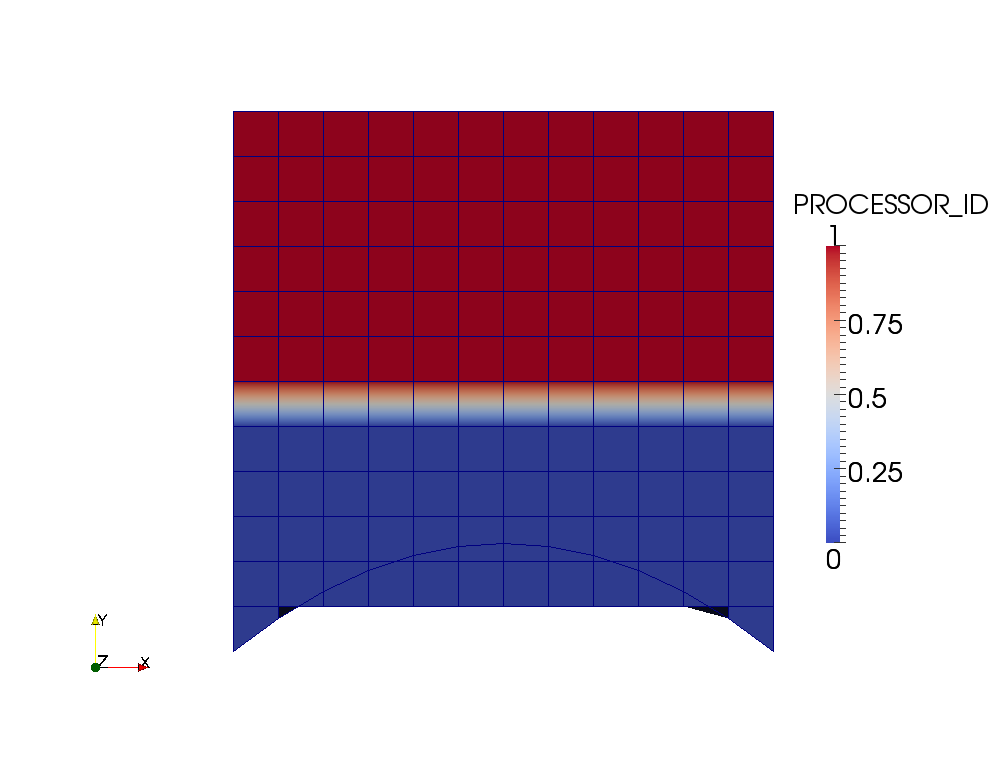
\includegraphics[width=4in]{figures/par-quad-orig}
\caption{Initial, tangled quadrilateral mesh.}
\label{fig:par_quad_orig}
\end{center}
\end{figure*}

\begin{figure*}[htpb]
\begin{center}
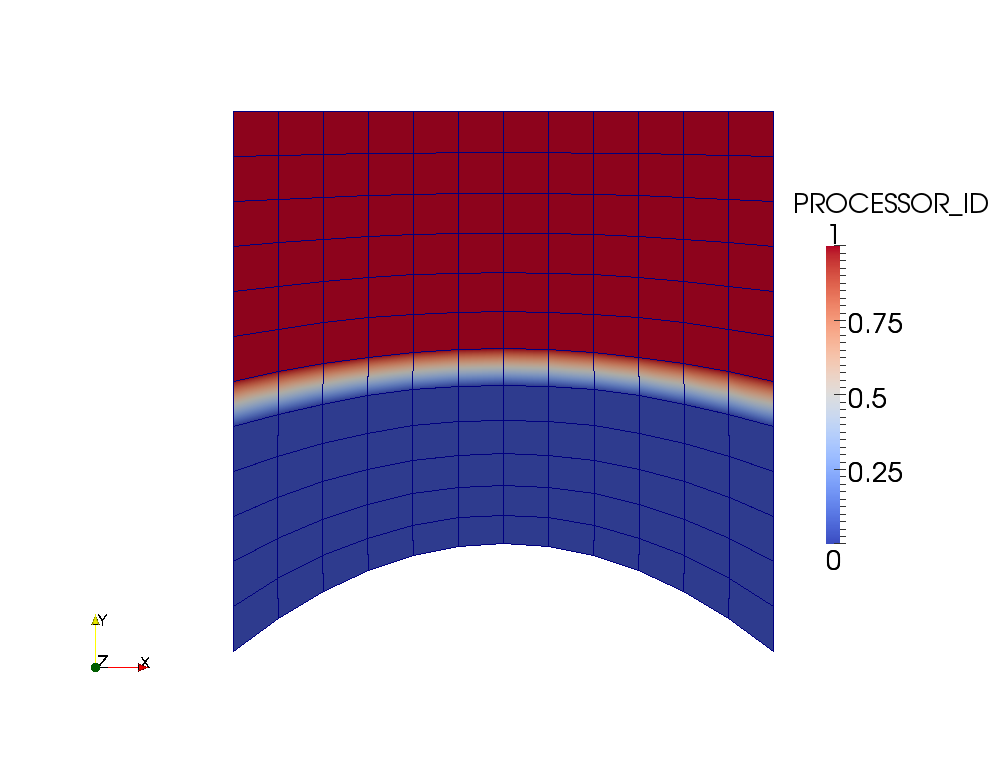
\includegraphics[width=4in]{figures/par-quad-smoothed}
\caption{Untangled and smoothed quadrilateral mesh.}
\label{fig:par_quad_smoothed}
\end{center}
\end{figure*}

\begin{figure*}[htpb]
\begin{center}
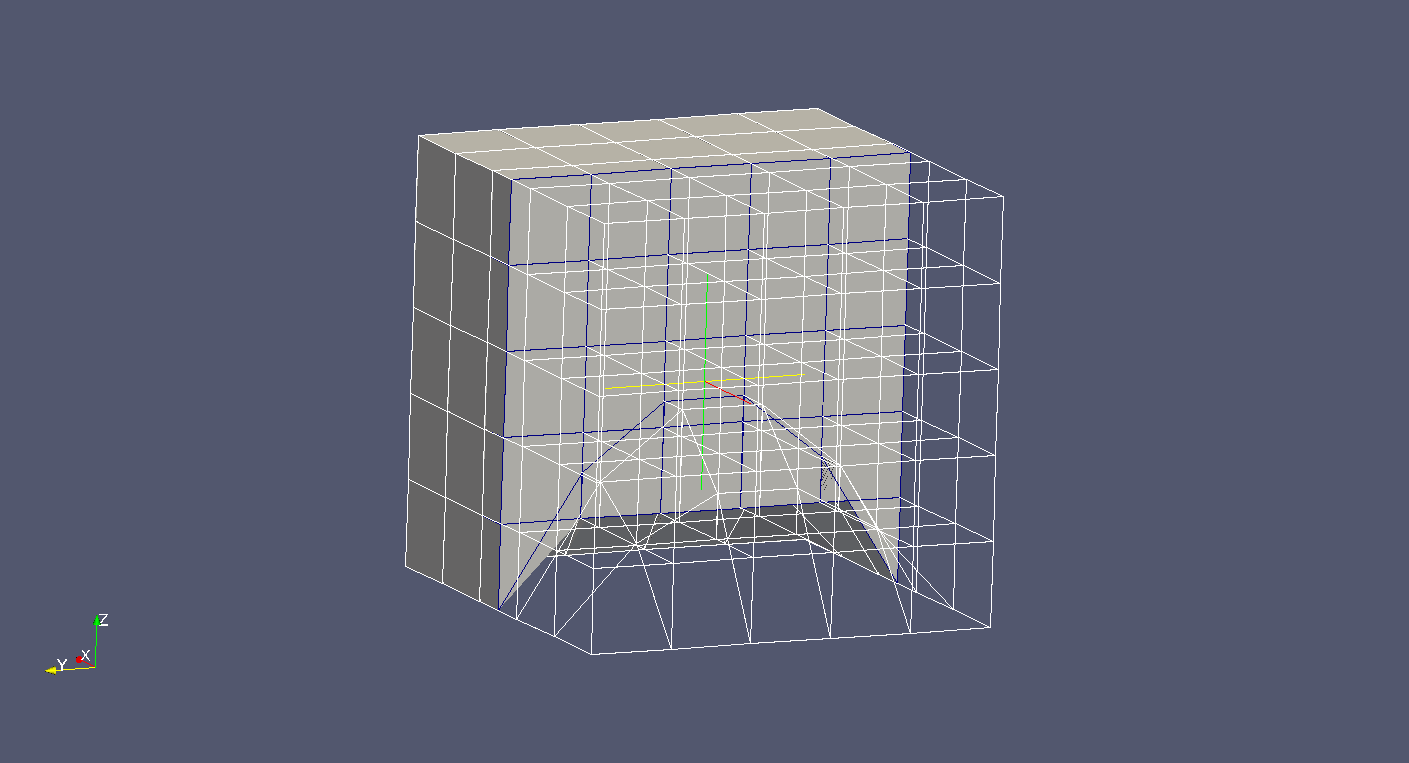
\includegraphics[width=4in]{figures/par-hex-orig}
\caption{Initial, tangled hexahedra mesh.}
\label{fig:par_hex_orig}
\end{center}
\end{figure*}

\begin{figure*}[htpb]
\begin{center}
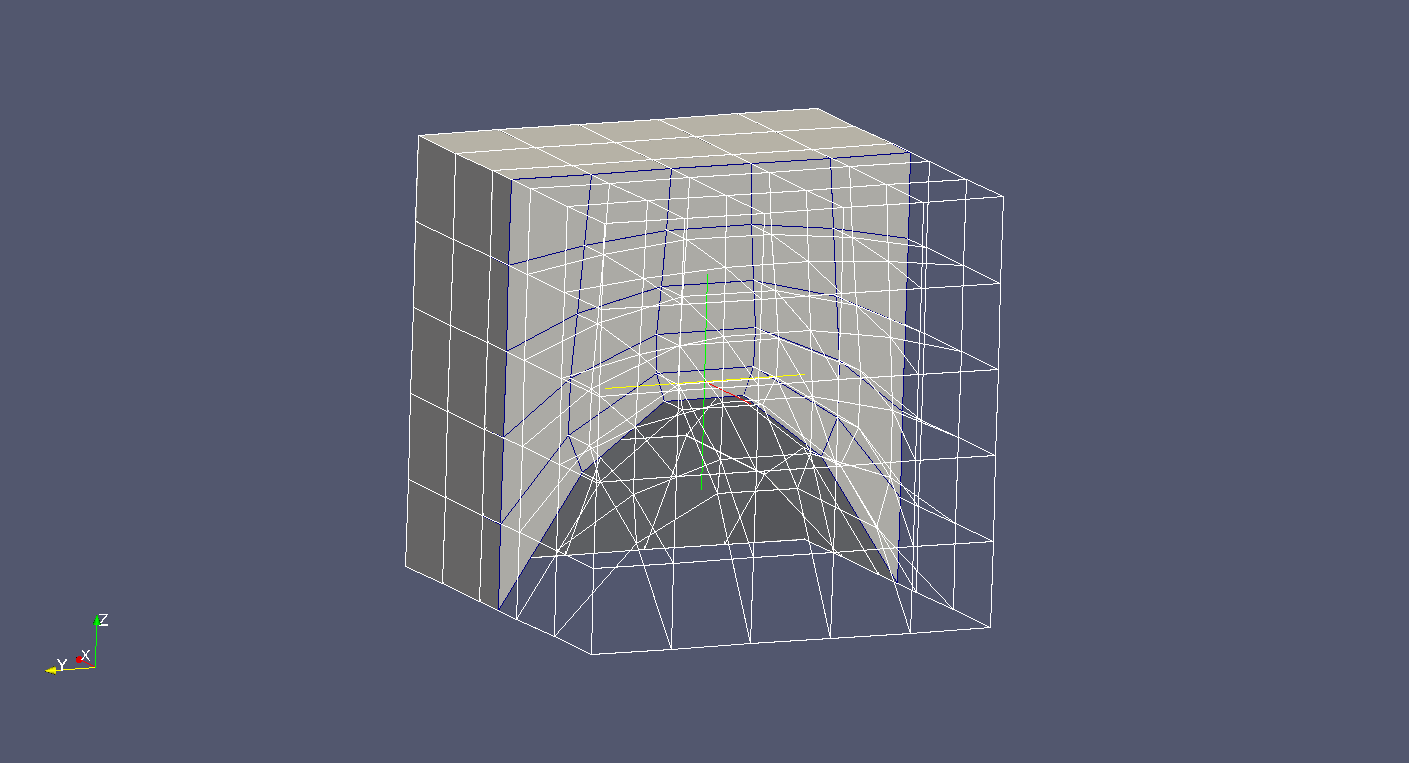
\includegraphics[width=4in]{figures/par-hex-smoothed}
\caption{Untangled and smoothed hexahedral mesh.}
\label{fig:par_hex_smoothed}
\end{center}
\end{figure*}

\subsection{Example: Using \texttt{Mesquite::Mesquite::MsqIMeshP}}

Similar to the example in Section \ref{sec:parallel-example-1}, this example uses the \texttt{LaplaceWrapper} wrapper in parallel to improve element shape.  However, this example assumes that either the iMeshP implementation is partitioning or that it is reading some pre-defined partitioned mesh and it relies on the iMeshP implementation to create ghost elements, assign global vertex IDs, etc.

An implementation of the iMesh and iMeshP APIs must be provided for this example to work.  Mesquite can use these APIs, but does not provide them.

\begin{verbatim}
/* Mesquite includes */
#include <Mesquite.hpp>
#include <MsqIMeshP.hpp>
#include <ParallelMeshImpl.hpp>
#include <ParallelHelper.hpp>
#include <MsqError.hpp>
#include <LaplaceWrapper.hpp>

/* other includes */
#include <mpi.h>
#include <iostream>
using namespace std;

int main( int argc, char* argv[] )
{
  const char input_file[] = "testmesh";
  const char output_file[] = "smoothmesh";

  /* init MPI */
  int rank, nprocs;
  if (MPI_SUCCESS != MPI_Init(&argc, &argv)) {
    cerr << "MPI_Init failed." << endl;
    return 2;
  }
  MPI_Comm_rank(MPI_COMM_WORLD, &rank);
  MPI_Comm_size(MPI_COMM_WORLD, &nprocs);

  /* create a new instance of the iMesh database */
  int ierr;
  iMesh_Instance mesh;
  iMesh_newMesh(NULL, &mesh, &ierr, 0);
  if (iBase_SUCCESS != ierr) return ierr;
  iBase_EntitySetHandle root_set;
  iMesh_getRootSet(mesh, &root_set, &ierr);
  if (iBase_SUCCESS != ierr) return ierr;

  /* create a partition instance in which to read
     the partitioned mesh */
  iMeshP_PartitionHandle partition;
  iMeshP_createPartitionAll(mesh, MPI_COMM_WORLD,
                            &partition, &err);
  if (iBase_SUCCESS != ierr) return ierr;

  /* load mesh */
  iMeshP_loadAll(mesh, partition, root_set, input_file,
                 NULL, &err, strlen(input_file), 0);
  if (iBase_SUCCESS != ierr) return ierr;

  /* create 1 layer of ghost entities */
  iMeshP_createGhostEntsAll(mesh, partition, 3, 1, 1, 0, &err);
  if (iBase_SUCCESS != ierr) return ierr;

  /* create MsqIMeshP instance */
  Mesquite::MsqError err;
  Mesquite::MsqIMeshP parallel_mesh(mesh, partition, root_set,
                                    iBase_REGION, err);
  if (err) {cerr << err << endl; return 1; }

  /* do Laplacian smooth */
  LaplaceWrapper optimizer;
  optimizer.run_instructions(&parallel_mesh, err);
  if (err) {cerr << err << endl; return 1; }

  /* write mesh */
  iMeshP_saveAll(mesh, partition, root_set, output_file,
                 NULL, &ierr, strlen(output_file), 0);
  if (iBase_SUCCESS != ierr) return ierr;

  /* cleanup */
  iMeshP_destroyPartitionAll(mesh, partition, &ierr);
  if (iBase_SUCCESS != ierr) return ierr;
  iMesh_dtor(mesh, &ierr);
  if (iBase_SUCCESS != ierr) return ierr;
  MPI_Finalize();
  return 0;
}
\end{verbatim}
